\documentclass[tikz,border=10pt]{standalone}
\usepackage{tikz}
\usetikzlibrary{arrows.meta, positioning}
\begin{document}
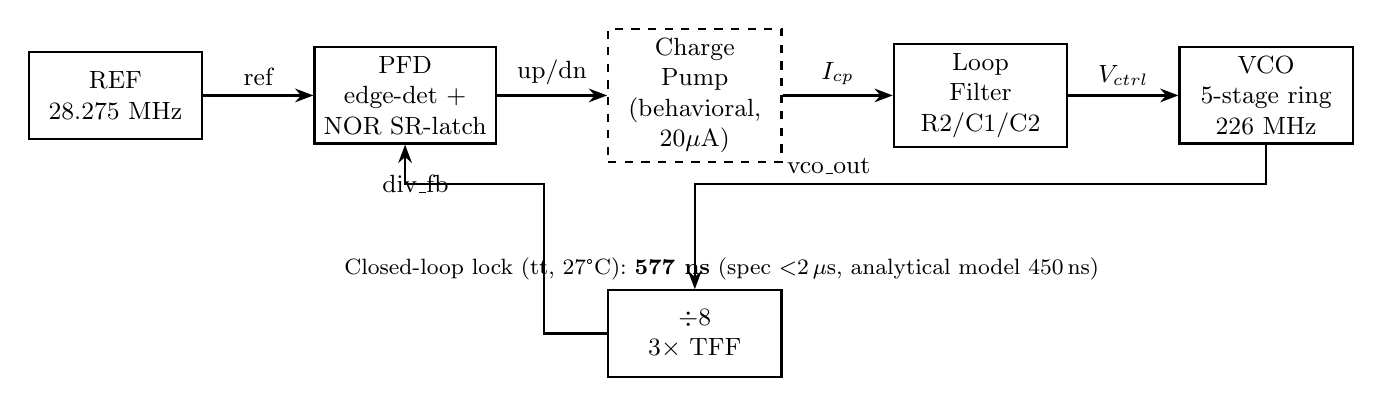
\begin{tikzpicture}[
  block/.style={draw, thick, minimum width=2.2cm, minimum height=1.1cm, align=center, font=\small},
  idealblock/.style={block, dashed},
  >=Stealth, thick, font=\small
]
\node[block] (ref) {REF\\28.275 MHz};
\node[block, right=1.4cm of ref] (pfd) {PFD\\edge-det +\\NOR SR-latch};
\node[idealblock, right=1.4cm of pfd] (cp) {Charge\\Pump\\(behavioral,\\20$\mu$A)};
\node[block, right=1.4cm of cp] (lf) {Loop\\Filter\\R2/C1/C2};
\node[block, right=1.4cm of lf] (vco) {VCO\\5-stage ring\\226 MHz};

\node[block, below=1.6cm of cp] (div) {$\div 8$\\3$\times$ TFF};

\draw[->] (ref) -- (pfd) node[midway, above]{ref};
\draw[->] (pfd) -- (cp) node[midway, above]{up/dn};
\draw[->] (cp) -- (lf) node[midway, above]{$I_{cp}$};
\draw[->] (lf) -- (vco) node[midway, above]{$V_{ctrl}$};
\draw[->] (vco.south) -- ++(0,-0.5) -| (div.north) node[midway, above, xshift=1.7cm]{vco\_out};
\draw[->] (div.west) -| ++(-0.8,1.9) -| (pfd.south) node[near start, left, xshift=-0.2cm]{div\_fb};

\node[align=center, font=\footnotesize] at (7.7,-2.2) {Closed-loop lock (tt, 27\textdegree C): \textbf{577 ns} (spec $<$2\,$\mu$s, analytical model 450\,ns)};
\end{tikzpicture}
\end{document}
